\section{Results and Tests}

\subsection{Driver}
The driver has full functionallity.
It recieves interrupts from the hardware via the OS and sends signals to the application.
It also cleans itself up as expected.

\subsection{Game}
In the end the game is a fully functioning puzzle game.
The game detects when there is no more places for new pieces and ends the game.
At the end of the game the score is shown and the gameboard is drawn red.

At this point of time the only button that works is SW6, and this button starts a new game.
The game works just as expected.

\subsection{Energy consumption}
For this assingment, the main focus was energy efficiency.
All the results describes the steps taken to improbe the energy efficiency of our game.

\subsubsection{Pausing on idle}
To prevent the game from exiting while idle we first did a polling.
This polling was interrupted on a signal and started right up again when the signal handler was done.
It was not energy efficent to wait and not do anything while using a lot of power.

To prevent this, we sat the game in full pause when waiting for input from the user.
This almost halved the power usage, and thus proved to be a much better solution.

Note that the images show the power usage when drawing the entire frame buffer at each input.

\begin{figure}[ht!]
    \begin{center}
    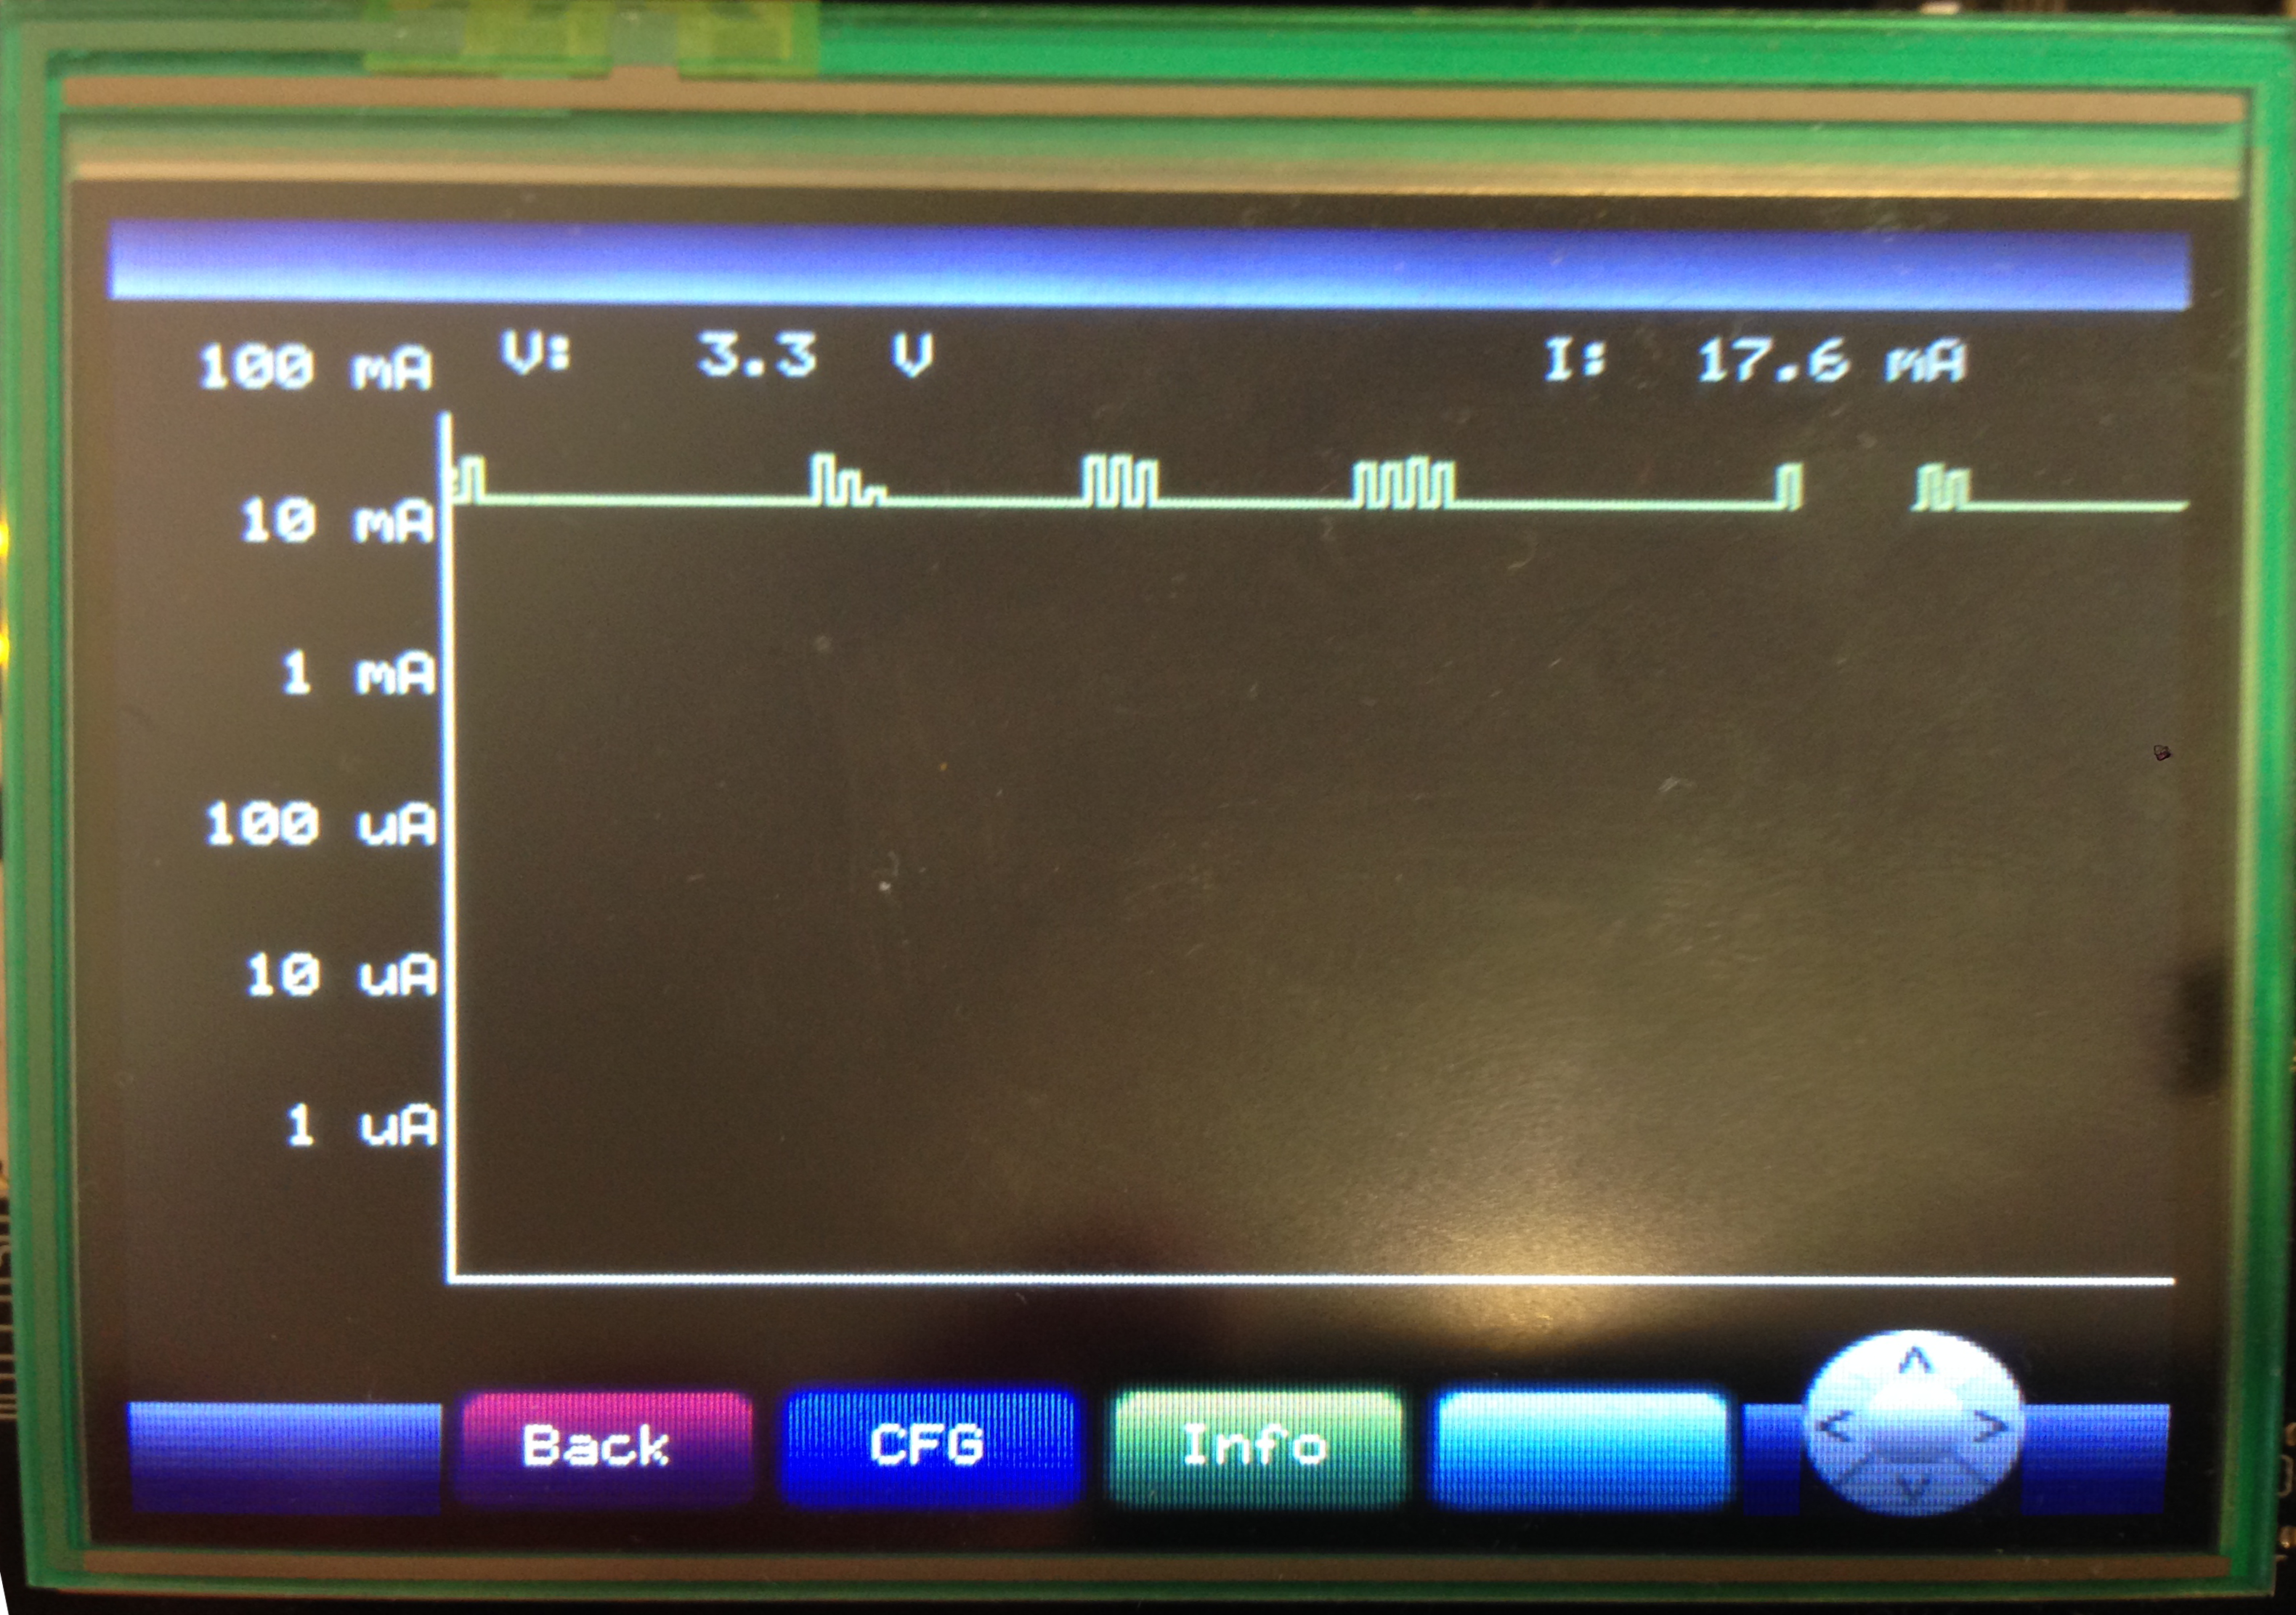
\includegraphics[scale=0.072]{assets/img/pre_pause.png}
    \caption{Power usage pre pauseing the game}
    \label{fig:idle}
    \end{center}
\end{figure}

\begin{figure}[ht!]
    \begin{center}
    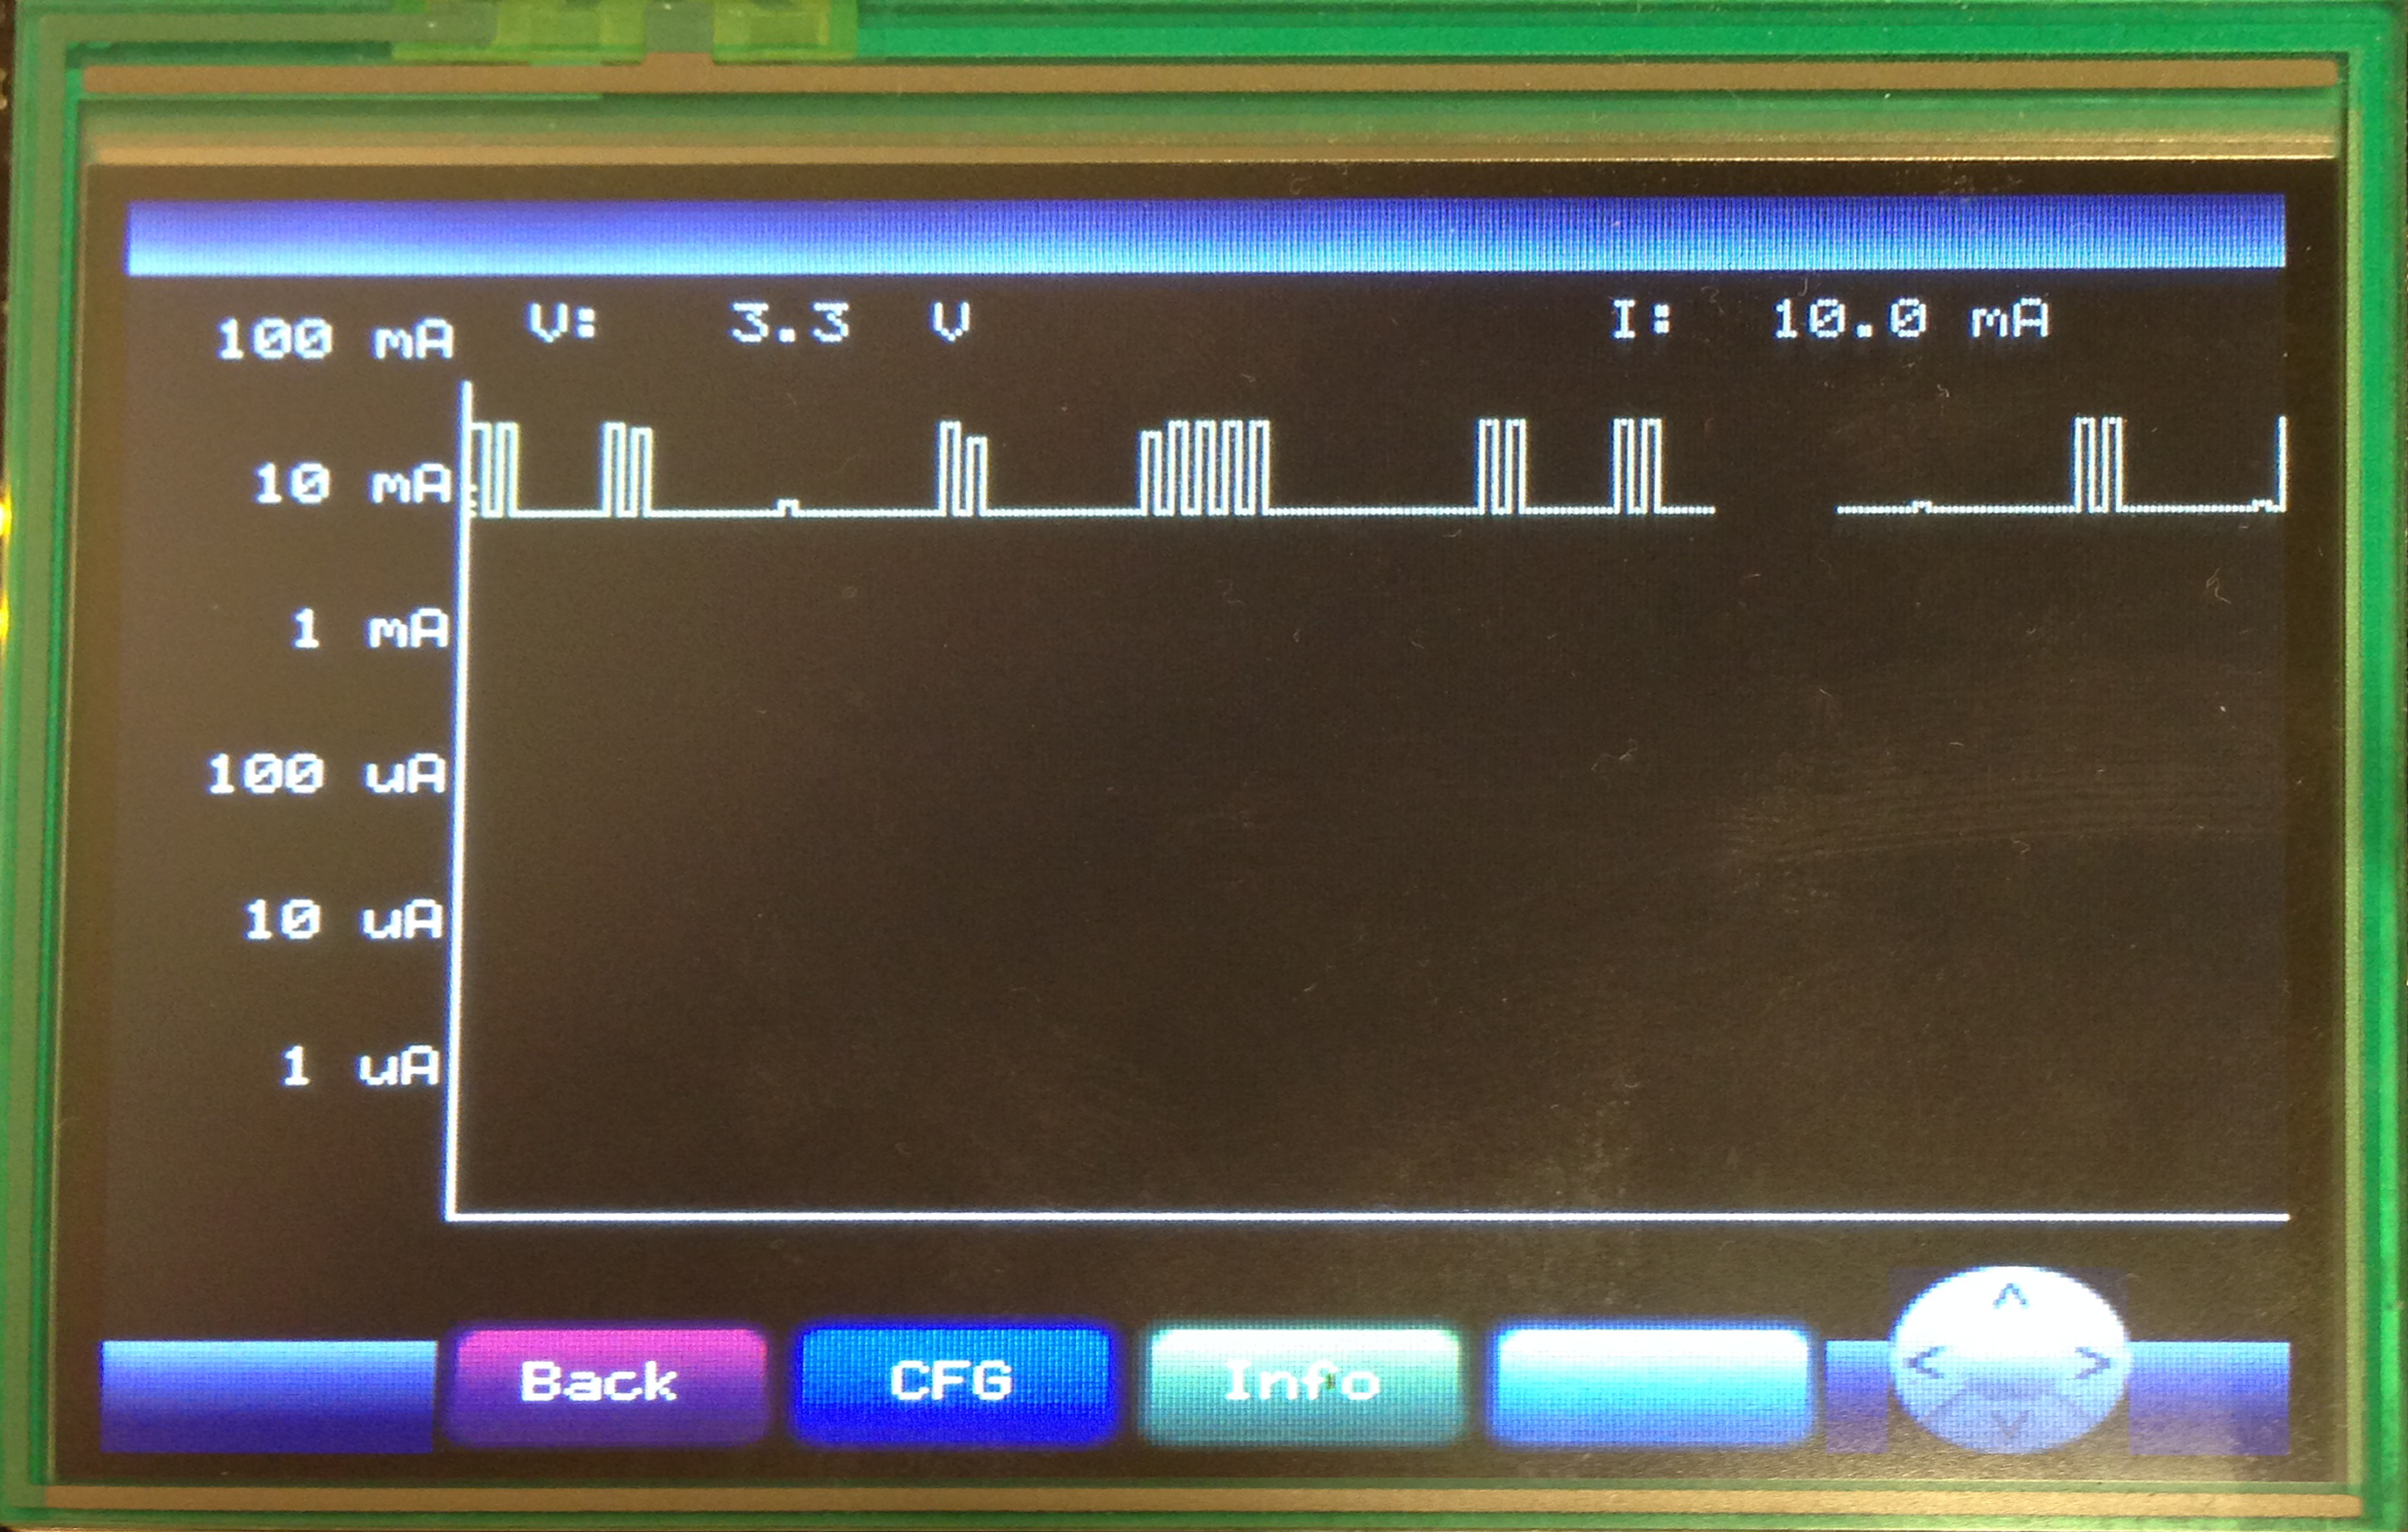
\includegraphics[scale=0.082]{assets/img/post_pause.png}
    \caption{Power usage post pauseing the game}
    \label{fig:idle}
    \end{center}
\end{figure}

\subsubsection{Drawing}
The drawing of the tiles on the screen was a big power hit.
It delayed the time the board could sleep, and cost a lot of energy.

At first, we re-drew the whole screen every time something happened.
The total time where the game didn't sleep was in this occasion 350 ms.
We then improved the sleeping-time and got it as low as 220 ms when only re-drawing the piece that was changed.
The first picture below shows the energy consumption when redrawing the whole screen, and the second picture shows the energy consumption when only redrawing parts.

\begin{figure}[ht!]
    \begin{center}
    \includegraphics[width=1\textwidth]{assets/img/waketime_full-redraw}
    \caption{Waketime on full redraw}
    \label{fig:idle}
    \end{center}
\end{figure}

\begin{figure}[ht!]
    \begin{center}
    \includegraphics[width=1\textwidth]{assets/img/waketime_delta-redraw}
    \caption{Waketime on only nessesary redraw}
    \label{fig:idle}
    \end{center}
\end{figure}
